
\begin{titlepage}
    % Strona tytułowa
    \vbox to\textheight{\hyphenpenalty=10000
    \begin{center}
	\begin{tabular}{p{107mm} p{9cm}}
	    \begin{minipage}{9cm}
	      \begin{center}
	      Politechnika Warszawska \\
	      Wydział Elektroniki i~Technik Informacyjnych \\
	      Instytut Informatyki
	      \end{center}
	    \end{minipage}
	    &
	    \begin{minipage}{8cm}
	    \begin{flushleft}
	     \footnotesize
	      Rok akademicki 2012/2013
	    \vspace*{2.75\baselineskip}
	    \end{flushleft}
	    \end{minipage} \\
	\end{tabular}
	\vspace*{3.75\baselineskip}
	\par\vspace{\smallskipamount}
	\vspace*{2\baselineskip}{\LARGE Praca dyplomowa inżynierska\par}
	\vspace{3\baselineskip}{\LARGE\strut Łukasz Rafał Szewczyk\par}
	\vspace*{2\baselineskip}{\huge\bfseries Projekt i~implementacja biblioteki dla Qt i~Qt~Quick do operowania na wykresach typu biurowego\par}

	\vspace*{7\baselineskip}
	\hfill\mbox{}\par\vspace*{\baselineskip}\noindent
	\begin{tabular}[b]{@{}p{3cm}@{\ }l@{}}
	    {\large\hfill } & {\large }
	\end{tabular}
	\hfill
	\begin{tabular}[b]{@{}l@{}}
	Opiekun pracy: \\[\smallskipamount]
	{\large mgr inż. Witold Wysota}
	\end{tabular}\par
	\vspace*{4\baselineskip}
    \begin{tabular}{p{\textwidth}}
    \begin{flushleft}
	\begin{minipage}{7cm}
	Ocena \dotfill
	\par\vspace{1.6\baselineskip}
	\dotfill
	\par\noindent
	\centerline{\footnotesize Podpis Przewodniczącego} \par
	\centerline{\footnotesize Komisji Egzaminu Dyplomowego}\par
	\end{minipage}
    \end{flushleft}
    \end{tabular}
    \end{center}}

    % Życiorys
    \newpage\thispagestyle{empty}
    \begin{tabular}{p{5cm} p{12cm}}
    \begin{minipage}{5cm}
    \center
    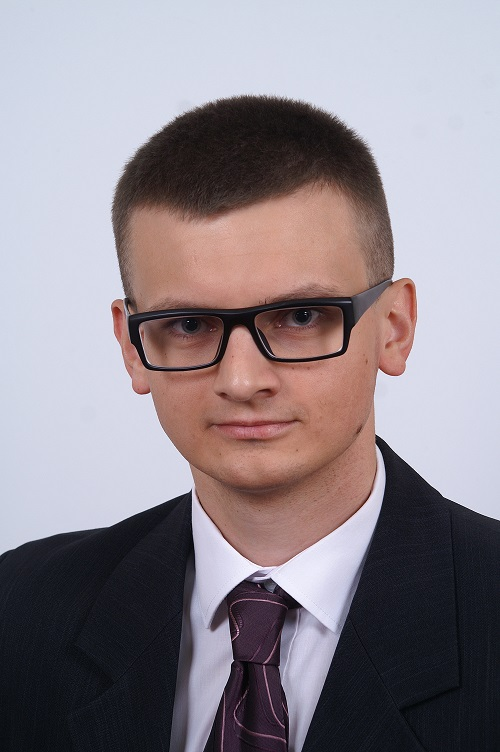
\includegraphics[height=6.5cm,width=4.5cm]{img/foto.jpg}
    \end{minipage}
    &
    \begin{minipage}{12cm}
    \begin{flushleft}
    \par\noindent\vspace{1\baselineskip}
    \begin{tabular}[h]{l l}
    {\normalsize\it Specjalność:} & Informatyka -- \\
    & Inżynieria systemów informatycznych
    \end{tabular}
    \par\noindent\vspace{1\baselineskip}
    \begin{tabular}[h]{l l}
    {\normalsize\it Data urodzenia:} & {\normalsize 02 grudnia 1990~r.}
    \end{tabular}
    \par\noindent\vspace{1\baselineskip}
    \begin{tabular}[h]{l l}
    {\normalsize\it Data rozpoczęcia studiów:} & {\normalsize 1 października 2009 r.}
    \end{tabular}
    \par\noindent\vspace{1\baselineskip}
    \end{flushleft}
    \end{minipage}
    \end{tabular}
    \vspace*{1\baselineskip}
    \begin{center}
	{\large\bfseries Życiorys}\par\bigskip
    \end{center}

    \indent
    Urodziłem się dnia 2. grudnia 1990 roku w~Warszawie. Całe dotychczasowe życie spędziłem mieszkając w~podwarszawskiej Kobyłce, w~której to uczęszczałem do szkoły podstawowej i~gimnazjum. Z~powodu zainteresowania matematyką zdecydowałem się w~roku 2006 rozpocząć naukę w~XVIII Liceum Ogólnokształcącym im. Jana Zamoyskiego w~Warszawie, w~klasie o~profilu matematyczno-fizyczno-informatycznym. W~pierwszej klasie liceum rozpocząłem równiez swoją przygodę z~siatkówką w~klubie Junior Stolarka Wołomin.
    \par
Dobre wyniki osiągnięte na egzaminach maturalnych w~roku 2009 pozwoliły mi dostać się na dzienne studia inżynierskie na Wydziale Elektroniki i Technik Informacyjnych Politechniki Warszawskiej.
W~trakcie studiów poza nauką kontynuowałem swój siatkarski rozwój, dzięki czemu trafiłem do zespołu AZS Politechnika Warszawska, który reprezentowałem w~rozgrywkach Młodej Ligi, przeznaczonych dla zawodników poniżej 23 roku życia, oraz w~rozgrywkach akademickich. W~2012 roku wróciłem do swojego macierzystego klubu, który w~międzyczasie wrócił do swojej historycznej nazwy -- Huragan Wołomin. W~sezonie 2012/13 udało mi się wywalczyć z~tym klubem awans do II ligi siatkówki.


    \par
    \vspace{2\baselineskip}
    \hfill\parbox{15em}{{\small\dotfill}\\[-.3ex]
    \centerline{\footnotesize podpis studenta}}\par
    \vspace{3\baselineskip}
    \begin{center}
 	{\large\bfseries Egzamin dyplomowy} \par\bigskip\bigskip
    \end{center}
    \par\noindent\vspace{1.5\baselineskip}
    Złożył egzamin dyplomowy w dn. \dotfill
    \par\noindent\vspace{1.5\baselineskip}
    Z wynikiem \dotfill
    \par\noindent\vspace{1.5\baselineskip}
    Ogólny wynik studiów \dotfill
    \par\noindent\vspace{1.5\baselineskip}
    Dodatkowe wnioski i uwagi Komisji \dotfill
    \par\noindent\vspace{1.5\baselineskip}
    \dotfill

    % Streszczenie
    \newpage\thispagestyle{empty}
    \vspace*{2\baselineskip}
    \begin{center}
	{\large\bfseries Streszczenie}\par\bigskip
    \end{center}

    {\itshape
    Praca prezentuje projekt biblioteki zawierającej uniwersalny silnik służący do tworzenia  biurowych wykresów w~Qt oraz Qt~Quick. Wykresy te są w~szczególności nastawione na interakcję z~użytkownikiem oraz współpracę z~już istniejącymi mechanizmami Qt.
	W~ramach pracy wykonano opis i~analizę wymagań oraz projekt architektury biblioteki. Zaplanowano również testy tworzonej biblioteki. Projekt zakłada implementację z~wykorzystaniem języka C++ oraz bibliotek Qt w~wersji 5.
	}
    \vspace*{1\baselineskip}

    \noindent{\bf Słowa kluczowe}: {\itshape uniwersalny silnik wykresów, obiektowa architektura.}
    \par
    \vspace{4\baselineskip}
    \begin{center}
	{\large\bfseries Abstract}\par\bigskip
    \end{center}
    \noindent{\bf Title}: {\itshape Project and implementation of office type charts library for Qt and Qt Quick}\par
    \vspace*{1\baselineskip}
    {\itshape
    This paper presents a~project of library containing universal engine for creating office charts in Qt and Qt~Quick. These plots are particularly focused on the user interaction and collaboration with existing mechanisms in Qt.
The paper contains description and~analysis of requirements and project of architecture of library. Also planned tests of designed library. The project involves the implementation using C++ language and Qt libraries in version 5.}
    \vspace*{1\baselineskip}

    \noindent{\bf Key words}: {\itshape universal charting engine, object oriented architecture.}

\end{titlepage}

% ex: set tabstop=4 shiftwidth=4 softtabstop=4 noexpandtab fileformat=unix filetype=tex spelllang=pl,en spell:
